\documentclass{article}
\title{Final Project: Face detector}
\author{Brendan Miller}
\date{March 12 2012}
\usepackage{multirow,amsmath}
\usepackage{graphicx}
\usepackage{fancyvrb}
\usepackage{color}
\usepackage{amsfonts}
\usepackage{hyperref}
\begin{document}
\maketitle

\begin{abstract}
A face detector implemented via a simplified Viola Jones algorithm.
\end{abstract}

\section{Project Overview}

For this project I implemented an binary image classifier that selects
faces from non-faces. This is based on the work of Paul Viola and
Michael Jones\cite{violajones2001}.

In the original Viola Jones paper, features were extracted from images
by first generating what they termed an integrated image. From the
integrated image, a large number of real valued features, described more fully in
the next section, could be computed quickly.

Given a large set of real valued features, a weak learner is
constructed by selecting a single feature and a threshhold value for
the feature that partitions example images into face and non-face
classes. This weak learner is conceptually similar to a decision tree
stump, although the metric used to find the optimal feature and
threashhold is different.

The weak learner is discussed more fully in section \ref{sec:weaklearner}.

Weak learners are combined with boosting (see section
\ref{sec:boosting}) in order to increase accuracy.

Finally, in the original Viola Jones paper, boosted classifiers were
combined in a cascade. The cascade was designed to reduce the
incendence of false positives, and to increase the performance of the
final classifer and possibly of the training phase. For my project I
have ommitted the cascade, as I said I would in my original project
proposal.

Even without the cascade, I've managed to achieve very high accuracy,
upwards of 99\%\footnote{Note this is on a validation set selected
  from the images provided with the project. I would expect accuracy
  to drop on images from a less carefully curated source.}, using a
boosted classifier over the features described in the original Viola
Jones paper.

\section{Feature Extraction}

\begin{figure}
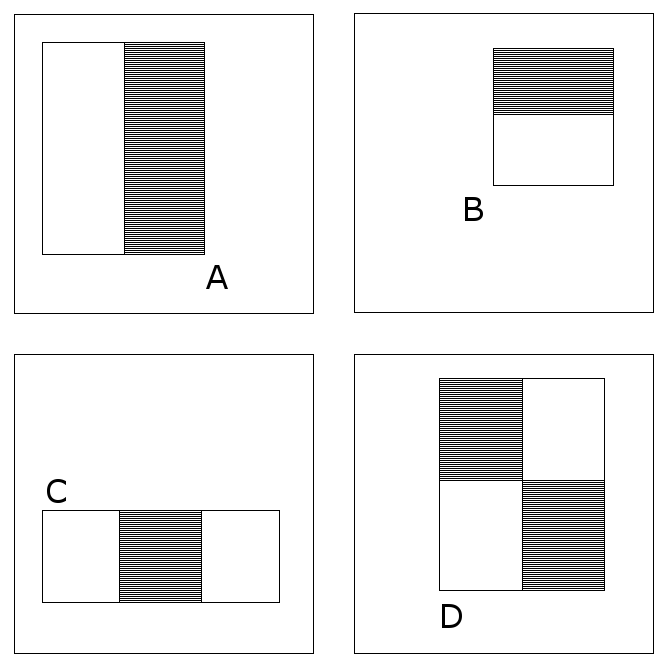
\includegraphics[width=40mm]{features.png}
\caption{Image features used to train the weak learner.}
\label{fig:features}
\end{figure}

The underlying features used to train the weak classifier are
illustrated in figure \ref{fig:features}\footnote{image from
  wikipedia}. These rectangular features are computed by summing
values of the pixels under the greyed out section, and subtracting the
sum of the pixels under the white section to produce a real valued
feature. For each feature type, a feature for every possible scale and
translation over the image are computed.

Rapid computation of these features probably the most important
innovation in Viola Jones. As discussed in the Viola Jones
2001\cite{violajones2001}, other detectors provide similar levels of
accuracy, but Viola Jones provides greatly improved performance.

To rapidly classify images, and also to provide more reasonable
training speeds, the features discussed in this paper can be quickly
computed by first creating an integral image. The integral image is of
the same dimension of the source image, but every element of the
integral image is the sum of all pixels above and to the left of that
coordinate in the source image.

From this integral image, the sum of a rectangular area can be
computer with only 4 array references, one to each corner of the
rectangle. A little algebra will similarly allow features A, B, C, and
D to be computed with a small number of references.

Even using the integrated image, the performance of feature
computation can be a drag on the algorithm. Especially in training on
large datasets, when millions of features need to be computed, it is
extremely important that feature computation is fast. For this reason,
after finding my initial pure python implementation to be too slow, I
rewrote the feature extraction code in C++, which made training go about 5 times as fast.

Another optimization that benefits the speed of training, but not of
classification, is to precompute all features and store them in main
memory. Originally I implemented my training stage this way, but found
that on large datasets the number of precomputed features was too
large to fit in main memory on a 32 bit machine.

For a 16 by 16 image, in my implementation there are 26944
features. Given 6000 training examples and 4 bytes per feature,
roughly 154 gigabytes of memory are necessary to precompute all the
features. Currently this is not practical.

\section{Weak Learner}
\label{sec:weaklearner}

\section{Boosted Classifier}
\label{sec:boosting}

\section{Experimental Results}

\section{Future Directions}

Training of weak learners is fairly parallelizable using fork join
parallelism. 

\begin{thebibliography}{9}

\bibitem{violajones2001}
  Paul Viola, Michael Jones\\
  Rapid Object Detection using a Boosted Cascade of Simple Features\\
  \url{http://research.microsoft.com/en-us/um/people/viola/Pubs/Detect/violaJones_CVPR2001.pdf}

\end{thebibliography}

\end{document}